\begin{figure}[htbp]\centering
\caption[Layer selection for the refusal-outcome audit]{Selecting a residual-stream index for the subsequent audit. Each point averages three model-specific AUCs: estimate a direction on one label-stratified half and rank outcomes on the other, using the same split at every index. The curve levels off after index 14; index 22 is the highest of the nine checked values. The orange marker shows that choice, not an independently validated optimal layer.}
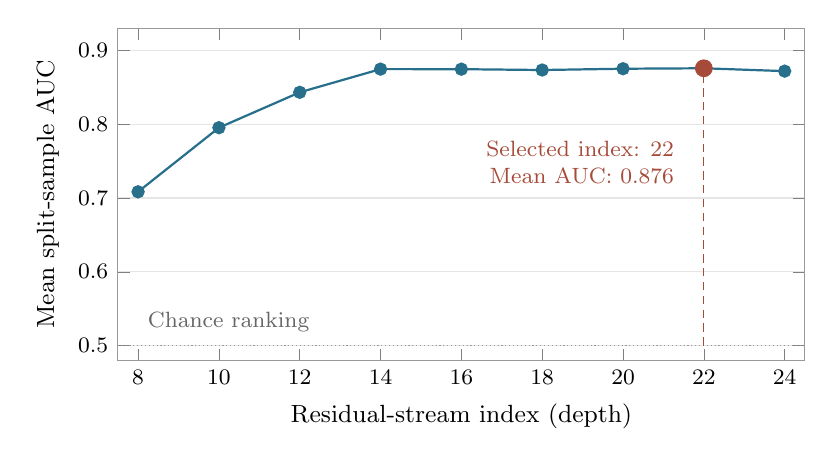
\begin{tikzpicture}
\definecolor{layerblue}{HTML}{286F8C}\definecolor{layerorange}{HTML}{A64B39}
\begin{axis}[width=.85\linewidth,height=5.8cm,xmin=7.5,xmax=24.5,ymin=.48,ymax=.93,xtick={8,10,12,14,16,18,20,22,24},ytick={.5,.6,.7,.8,.9},xlabel={Residual-stream index (depth)},ylabel={Mean split-sample AUC},label style={font=\small},tick label style={font=\footnotesize},axis line style={black!40},ymajorgrids,grid style={black!10}]
\addplot[black!40,densely dotted] coordinates {(7.5,.5)(24.5,.5)};
\addplot[thick,color=layerblue,mark=*,mark size=2pt] coordinates {(8,0.7083884479717814) (10,0.7952374790495909) (12,0.8431731790945042) (14,0.8745912616254232) (16,0.8745210846013124) (18,0.8733831898298773) (20,0.8751263186433994) (22,0.8757466150711491) (24,0.871869077743819)};
\draw[densely dashed,layerorange] (axis cs:22,.5) -- (axis cs:22,0.8757466150711491);
\addplot[only marks,mark=*,mark size=3pt,color=layerorange] coordinates {(22,0.8757466150711491)};
\node[font=\footnotesize,align=right,anchor=north east,text=layerorange] at (axis cs:21.5,.79) {Selected index: 22\\Mean AUC: 0.876};
\node[font=\footnotesize,anchor=south west,text=black!60] at (axis cs:8,.505) {Chance ranking};
\end{axis}\end{tikzpicture}
\label{fig:mechanistic-layer-sweep}\fonte{Author.}\end{figure}
